%! TEX program = xelatex
\documentclass{report}
\usepackage[UTF8, scheme= plain]{ctex}
\usepackage{fancyhdr}
\usepackage{tocloft}
\usepackage[margin=1in]{geometry}
\usepackage{metalogo}                   % \XeLaTeX
\usepackage{float}                      % figure H flag
\usepackage{microtype}                  % break long words
\usepackage[bottom]{footmisc}           % force footnote stay bottom
\usepackage{listings}                   % code
\usepackage{xparse}                     % newcommand multiple optional arguments
\usepackage[hidelinks]{hyperref}
\usepackage{tabularx}
\usepackage{enumitem}
\usepackage{algorithm}                  % algorithm pseudo code
\usepackage{algpseudocode}
\usepackage{caption}
\usepackage{amsmath}                    % advanced math support
\usepackage{lmodern}                    % allow font to scale

% make chapter stay in the same page
%\makeatletter
%\renewcommand\chapter{\thispagestyle{plain}%
%\global\@topnum\z@
%\@afterindentfalse
%\secdef\@chapter\@schapter}
%\makeatother
% settings %%%%%%%%%%%%%%%%%%
%%%%%%%%%%%%%%%%%%%%%%%%%%%%%
%\ctexset{
%    chapter = {
%        format += \flushleft,
%        number = \Roame{chapter},
%        name = {Part},
%    },
%    section = {
%        format += \flushleft,
%    },
%    appendix = {
%        number = \Alph{chapter},
%        name = {Appendix},
%    },
%}

\pagestyle{fancy}
\setlength\cftaftertoctitleskip{2em}
\graphicspath{{./res/}}

% defines %%%%%%%%%%%%%%%%%%%
%%%%%%%%%%%%%%%%%%%%%%%%%%%%%
%\newfontfamily\codeF{Fira Code}
\DeclareDocumentCommand{\inputCode}{ O{c} m }{
    {
        \setmainfont{FiraCode Nerd Font}[
            ItalicFont  = FiraCode Nerd Font
        ]
        \lstinputlisting[
            basicstyle=\codeF,
            language=#1,
            tabsize=4,
            showstringspaces=false,
            breaklines=true,
            frame=shadowbox,
            framexleftmargin=10mm,
            rulesepcolor=\color{black},
            basicstyle=\small,
            numbers=left,
        ]{#2}
    }
}

\NewDocumentEnvironment{simpleAlgorithm}{m}
{
\captionof{algorithm}{#1}
\hrule
\begin{algorithmic}[1]
} {
\end{algorithmic}
\hrule \vspace{1em}
}
\renewcommand{\baselinestretch}{1.5}
% report content %%%%%%%%%%%%
%%%%%%%%%%%%%%%%%%%%%%%%%%%%%
\begin{document}
\begin{titlepage}
    \addtolength{\topmargin}{1cm}
    \centering
    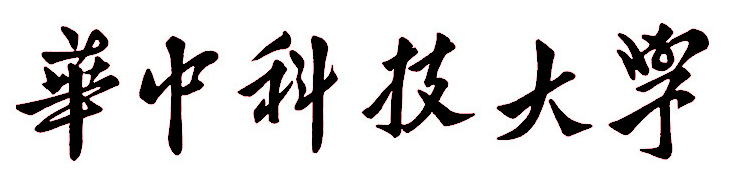
\includegraphics[width=0.6\textwidth]{hust.jpg}\par
    \vspace{1cm}
    {\Huge A Simple Crash-tolerant Consensus Implementation Using Raft}\par
    \vspace{10cm}
    {
        \large
        \begin{tabular}{r m{10em}}
            \makebox[7em][s]{Team Member 1}:& Sixu Hu(胡思勖)\\ \cline{2-2}
            \makebox[7em][s]{Email address}:&  husixu1@hotmail.com\\ \cline{2-2}
            \makebox[7em][s]{Team Member 2}:& Yifu Deng(邓一夫)\\ \cline{2-2}
            \makebox[7em][s]{Email address}:&  deng3652@gmail.com\\ \cline{2-2}
            \makebox[7em][s]{Team Member 3}:& Junhua Zhang(张俊骅)\\ \cline{2-2}
            \makebox[7em][s]{Email address}:&  497387417@qq.com\\ \cline{2-2}
        \end{tabular}
    }
    \vfill
    2018.01.01
\end{titlepage}

\setcounter{tocdepth}{1}
\tableofcontents
% Chapter 1 %%%%%%%%%%%%%%%%%
%%%%%%%%%%%%%%%%%%%%%%%%%%%%%
\chapter{Raft Algorithm Introduction}

\section{Consensus protocol}
Consistency means that multiple servers agree in state, but in a distributed system, because of various accidents, some servers may crash or become unreliable, and it can not reach a consistent state with other servers. This requires a consensus protocol, which is designed to ensure fault tolerance, that is, even if there are one or two servers in the system that do not impact its processing.

\section{Raft algorithm}
In a distributed database system, if each node has the same initial state and each node performs the same sequence of operations, then they eventually get a consistent state. To ensure that each node executes the same sequence of commands, it is necessary to execute a "consistency algorithm" on each instruction to ensure that the instructions seen by each node are consistent. And Raft is such an algorithm, we can use it to solve the problems.

\section{The protocol of Raft}
\begin{itemize}
\item Each replica of the agreement is in one of three states: Leader, Follower or candidate.
\item Leader is the processor of all requests, the replication of leader receives the client's update request, do local process and then synchronized to other copies.
\item Follower is passive updaters of the request, it receives update requests from leader, and then write to local logs. A follower does not take the initiative to initiate the request.
\item Candidate is the intermediate state from follower to leader conversion. when the follower replica does not receive a heartbeat from the leader replica for a period of time, then it shows that the leader may have failed. At this time, the election process is started and the replica becomes a candidate until the election is over.
\end{itemize}

\section{The details of Raft}
\subsection{Terms}
As we all know, in a distributed environment, time synchronization is a big problem, but in order to identify outdated information, time information is essential. To solve this problem, in raft algorithm, the time is divided into terms, a term can be considered a logical time.
\begin{itemize}
\item There is at most one leader per term.
\item In some terms, due to the failure of the election, there is no leader.
\item Every servers maintains current term locally.
\end{itemize}
\subsection{Heartbeats and Timeouts}
\begin{itemize}
\item All servers start as a follower, and start the election timer.
\item Follower expects to receive RPC from leader or candidates.
\item Leader must broadcast heartbeat to reset follower's election timer.
\item If the follower’s election timer times out, it assumes that the leader has crashed and then initiates a election.
\end{itemize}

\subsection{Leader election}
Increment by term, follower changes to candidate, set a vote for itself, initiate a RPC of requesting vote in parallel, and try again until one of the following conditions is met:
\begin{itemize}
\item Get over half votes of servers, then convert to leader, broadcasts heartbeat simultaneously.
\item Reveive legal RPC of append entries, then converted to follower.
\item Election timeout, no successful server election, increment by term and election again.
\end{itemize}

\subsection{Log replication}
The normal process:
\begin{itemize}
\item Client sends command to the leader.
\item Leader appends command to the local log.
\item Leader broadcasts the append entries RPC to followers.
\item Once the log entry committed successfully:\par
(1) The leader applies the corresponding command to the local state machine and returns the result to the client.\par
(2) The leader notifies committed log entries to follower through subsequent append entries RPC.\par
(3) If the follower receives the commit log entry, applies it to the local state machine.
\end{itemize}

\subsection{Safty}
In order to ensure the correctness of the whole process, the Raft algorithm guarantees that the following attribute are true:
\begin{itemize}
\item Election Safety\par
Within any given term, select up to one leader.
\item Leader Append-Only\par
The leader never rewrites or deletes the local log, just appends the local log.
\item Log Matching\par
If the log entries on both nodes have the same index and term, the logs in the two nodes [0, Index] are exactly the same.
\item Leader Completeness\par
If a log entry is committed in a term, then any subsequent term of leader owns the log entry.
\item State Machine Safety\par
Once a server applies a log entry to a local state machine, all subsequent server apply the same log entry for that offset.
\end{itemize}

\subsection{Other details}
\begin{itemize}
\item Candidate may receive append entries RPC from other leaders while waiting for the voting result. If the leader’s term is not less than the local current term, the legitimacy of the leader identity is recognized and proactively downgraded to follower; otherwise, the candidate identity is maintained and wait for a voting result.
\item Candidate has neither successful election nor received RPC from other leaders. It usually happens when multiple nodes initiate the election at the same time, and eventually each candidate will be timeout. In order to reduce the conflict, we shall use a strategy named random concession, it means each candidate restart the election timer as a random value, and then it greatly reduced the probability of conflict.
\end{itemize}

% Chapter 2 %%%%%%%%%%%%%%%%%
%%%%%%%%%%%%%%%%%%%%%%%%%%%%%

\chapter{Difference between Raft \& Paxos}

\section{Brief discription of two algorithms}
\begin{itemize}
\item Raft is a consensus algorithm for managing a replicated log designed by Diego Ongaro and John Ousterhout, Stanford University. It produces a result equivalent to (multi-)Paxos, and it is as efficient as Paxos, but its structure is different from Paxos; this makes Raft more understandable than Paxos and also provides a better foundation for building practical systems.
\item Paxos and Raft are called consensus protocols. As the name implies, they address the issue of multi-node consensus. It should be noted that the consensus mentioned here does not mean that all nodes are in exactly the same state at any moment, but to ensure that: even in the event of network partition or machine node anomalies, the entire cluster can still provide a consistent service, that is, each operation can see that all previous successful operations are completed in sequence.
\end{itemize}

\section{Different difficulty}
The advantages of the Raft protocol over Paxos are that Raft is easier to understand and implement. It strengthens the leader's position, and the entire protocol can be clearly divided into two parts, and uses the continuity of the log to do some simplification:
\begin{itemize}
\item When the leader is running normally, it synchronizes the log of followers.
\item When the leader is crashed, choose a new leader.
\end{itemize}

\section{Different process}
Multi-paxos and Raft both use a number to identify the leader, multi-paxos called proposer-id, Raft called term, the meaning is the same. In Multi-paxos, the leader which has the biggest proposer-id can commit an effective resolution. In Raft protocol ,  the unique node whose term is the biggest can be the leader. The distinction leader’s legitimacy strategy of Multi-paxos is the same as Raft. Whose proposer-id is larger, who is legal, and the proposer-id is the only. Therefore, in fact, at the same time, they only have a valid leader. In the raft protocol leader election algorithm, the newly elected leader already has all the logs that can be committed, while multi-paxos does not need to guarantee this. This also means that multi-paxos needs extra flow to get the logs that have already been committed from other nodes. Therefore, the raft protocol log can simply flow from the leader to the follower, while multi-paxos requires additional processes to complete the committed log.

\section{Different log continuity}
Raft protocol emphasizes the continuity of the log, but multi-paxos allows the log is not continuous. The continuity of the log contains such a nature: If two different nodes have the same sequence of logs, as long as the term is the same, the two logs must be the same, and it must be same with the previous log. This makes it convenient that when the leader wants the follower to synchronize the log. At the same time, log commit of Raft protocol is also continuous. If a log is committed, all the logs before the log are committed. If a log can be committed, all the logs before it can be committed. This also guarantees that when the Raft protocol is elected for the leader, a node in the majority must have all the committed logs. This is because that the last committed log is recorded by at least the majority. Due to the log continuity, having a log for the last commit means having all the commit logs, that is, at least one majority has all committed logs. For multi-paxos, it allows the log is not continuous. Each log need to be confirmed that if it can be individually committed. So when a new leader is generated, it has to reconfirm each uncommitted log to determine if they can be committed. Even the new leader may miss the logs that can be committed and need to get the missing committable logs from other nodes through the Paxos phase 1. So essentially, the two protocols are the same. If a log is owned by the majority, then it can be committed, but the leader needs to know this in some way. In the meantime, in order for the log that has been committed to not be overwritten by the new leader, the new leader needs to have all the logs that have been committed(or can be committed) to make it works normally. The difference between the two is the way that the leader confirms committing and gets all the logs that can be committed, and the difference is due to whether the logs are consistent or not. The Raft protocol uses log continuity to simplify the process.


% Chapter 3 %%%%%%%%%%%%%%%%%
%%%%%%%%%%%%%%%%%%%%%%%%%%%%%

\chapter{Mechanism of Raft}


\section{A brief discription of Raft}
There are three types of roles in a cluster organized by the Raft protocol: Leader, Follower and candidate.\par
The state changes of this three types of character changes are as shown in figure \ref{fig:state}.
\begin{figure}[H]
    \centering
    \includegraphics[width=0.7\linewidth]{state.png}
    \caption{The state changes of them}
    \label{fig:state}
\end{figure}

\section{The process of election}
Let us give a simple example. As shown in figure \ref{fig:vote}, a minimum Raft democratization requires three participants (pictured below: A, B, C) so that a majority of votes exists. A, B and C are all followers by the initial state, and then launched one election of the three possible situations. 
The first two in the picture below can all be chosen as leader. The third one shows that this round of voting is invalid (Split Votes): each side has voted for itself. As a result, no one obtains the majority vote. After that, each participant randomly elected for the Election Timeout to re-initiate the voting until one party won the majority vote. The first from the timeout to resume the voting in the direction of the other two are still timeout request for a vote, then they can only vote for each other, and soon reached an agreement.
\begin{figure}[H]
    \centering
    \includegraphics[width=0.7\linewidth]{vote.png}
    \caption{vote states}
    \label{fig:vote}
\end{figure}
If a leader is selected, leader maintains its dominance by sending regular heartbeat messages to all followers. If a follower did not receive the leader's heartbeat for a period of time, it is assumed that the leader may have been crashed and started the election process again.


\section{Impact of the leader node on consensus}
Let's discuss the impact of leader nodes on consistency. The Raft protocol strongly depends on the availability of leader nodes to ensure the consistency of cluster data. As shown in figure \ref{fig:total}, the flow of data can only be transferred from the leader node to the follower node. After the data is submitted to the cluster leader node, the data received by the leader node is in a uncommitted state. The Leader node then concurrently replication data to all the follower nodes and waits for the receiving response, ensuring that at least half of the nodes in the cluster have received after the data to the client to confirm the data has been received. Once the data is sent to the client to receive the ACK response, it indicates that the data status has been committed. The leader node then notifies the follower node that the data status has been submitted.
\begin{figure}[H]
    \centering
    \includegraphics[width=0.7\linewidth]{total.png}
    \caption{Total process diagram}
    \label{fig:total}
\end{figure}
During this process, the master node may crash at any stage. Let’s see how the Raft protocol guarantees data consistency for different stages.

\section{The process of Raft}
\subsection{Before data arrives at the leader node}
As shown in figure \ref{fig:1}, leader crash does not affect consistency at this stage.
\begin{figure}[H]
    \centering
    \includegraphics[width=0.7\linewidth]{1.png}
    \caption{Process diagram}
    \label{fig:1}
\end{figure}

\subsection{Data arrives at the leader node but not replicated to the follower node}
 As shown in figure \ref{fig:2}, leader crashed at this stage, the data is uncommited state. Client will not receive Ack, it will think timeout failed, and can safely initiate a retry. Follower nodes do not have the data, after re-select the new leader, client retry to re-submit successfully. After the original leader node is recovered, it joins the cluster as a follower, synchronizes the data from the new leader of the current term, and enforces the consistency with the leader data.
\begin{figure}[H]
    \centering
    \includegraphics[width=0.7\linewidth]{2.png}
    \caption{Process diagram}
    \label{fig:2}
\end{figure}


\subsection{The data arrives at the leader node, successfully replicated to all follower nodes, but has not yet response to the leader}
As shown in figure \ref{fig:3}, leader crashed at this stage, although the data in the follower node is in the uncommitted state but consistent. the data can be committed after Re-electing the leader. At this time, client does not know whether it has been committed successfully, it can retry commit. In this case, Raft requires that RPC requests be idempotent, that is, to implement the internal deduplication mechanism.
\begin{figure}[H]
    \centering
    \includegraphics[width=0.7\linewidth]{3.png}
    \caption{Process diagram}
    \label{fig:3}
\end{figure}

\subsection{The data arrives at the leader node, successfully replicated to a part of follower nodes, but has not yet response to the leader}
As shown in figure \ref{fig:4}, leader crashed at this stage, the data in the follower node is in the uncommitted state and not consistent. The Raft protocol requires that votes be cast only to nodes that have the most recent data. So the node with the latest data will be selected as the leader and then forced to synchronize the data to follower, the data will not be lost and eventually consistent.
\begin{figure}[H]
    \centering
    \includegraphics[width=0.7\linewidth]{4.png}
    \caption{Process diagrams}
    \label{fig:4}
\end{figure}

\subsection{The data arrives at the leader node, successfully replicated to all or most follower nodes, the data in the leader is in the committed state, but the follower is in the uncommitted state}
As shown in figure \ref{fig:5}, leader crashed at this stage. After re-electing the new leader, the process is the same as in Phase 3.
\begin{figure}[H]
    \centering
    \includegraphics[width=0.7\linewidth]{5.png}
    \caption{Process diagram}
    \label{fig:5}
\end{figure}

\subsection{The data arrives at the leader node, successfully replicated to all or most follower nodes, the data is in the committed state at all nodes, but has not responsed to the client}
As shown in figure \ref{fig:6}, leader crashed at this stage. the internal data of the cluster is already consistent. Client repeat retries based on idempotent policies have no effect on consistency.
\begin{figure}[H]
    \centering
    \includegraphics[width=0.7\linewidth]{6.png}
    \caption{Process diagram}
    \label{fig:6}
\end{figure}

\subsection{Network partition led to double leader situation}
As shown in figure \ref{fig:7}, the network partition separates the original leader node from the follower node. The follower can not receive the heartbeat of the leader and will initiate the election to generate a new leader. At this time it has produced double leader, the original leader is alone in a district, the data submitted to it is impossible to be replicated to most nodes, so it cannot be submitted successfully. Submitting data to the new leader can be successful. After the network is recovered, the old leader discovers that there is a new leader with a new term in the cluster and it will automatically downgrad to follower, and the data is synchronized with the new leader to achieve the same cluster data.
\begin{figure}[H]
    \centering
    \includegraphics[width=0.7\linewidth]{7.png}
    \caption{Process diagram}
    \label{fig:7}
\end{figure}

\subsection{Summary}
To summarize, we exhaustively analyzed all the situations faced by the smallest cluster (3 nodes). It can be seen that the Raft protocol can well cope with the consensus problem and is easy to understand.

% Chapter 4 %%%%%%%%%%%%%%%%%
%%%%%%%%%%%%%%%%%%%%%%%%%%%%%

\chapter{A Simple Implementation of Raft}
\section{System structure}
As shown in figure \ref{fig:SYS}, we used a system structure diagram to describe our finished work, it roughly describes how this system works.
\begin{figure}[H]
    \centering
    \includegraphics[width=0.7\linewidth]{SYS.png}
    \caption{System structure diagram}
    \label{fig:SYS}
\end{figure}

\section{Main functions \& algorithms}
We chose several important functions as an example, and listed the flow charts and specific algorithms for these functions.
\subsection{startElection()}
This function begins when there is a timeout or at the start. There is not a valid leader in the network. Through this function, the node start a election, clear the vote status, become a candidate, and sending vote request to other nodes.
\subsubsection{Flow chart}
The flow chart of this algorithm shown in figure \ref{fig:SE}.
\begin{figure}[H]
    \centering
    \includegraphics[width=0.2\linewidth]{SE.png}
    \caption{Start election}
    \label{fig:SE}
\end{figure}

\subsubsection{Algorithm}
\begin{simpleAlgorithm}{follower starts a election}
    \Procedure{startElection}{}
    \State \Call{setCurrentTerm}{$currentTerm + 1$} \Comment{update current term}
    \For{$node \gets$ each node in network}
        \State $node.votedForMe \gets false$  \Comment{clear vote status}
    \EndFor
    \State \Call{voteFor}{$id,TRUE$} \Comment{vote for myself}
    \State $currentLeader \gets invalid$
    \State $state \gets stateCandidate$
    \For{$node$ = each node in network except myself}
        \If{$node \neq id$}
            \State \Call{requestVoteFrom}{$node.id$)}
        \EndIf
    \EndFor
    \State \Call{resetTimeout}{} \Comment{randomize election timeout to avoid forever loop}
   \EndProcedure
\end{simpleAlgorithm}


\subsection{receiveVoteRequest()}
When a node receives a vote request, It will determine whether its own term is smaller than the requesting node, and if so, it will be a follower and reset timeout. Then, it will call the function shouldVote to determine vote or not. Finally, it will reset timeout.
\subsubsection{Flow chart}
The flow chart of this algorithm shown in figure \ref{fig:RQ}.
\begin{figure}[H]
    \centering
    \includegraphics[width=0.6\linewidth]{RQ.png}
    \caption{Receive vote request}
    \label{fig:RQ}
\end{figure}

\subsubsection{Algorithm}
\begin{simpleAlgorithm}{node receives a vote request}
    \Procedure{receiveVoteRequest}{voteRequest}
    \If{$currentTerm < voteRequest.term$} \Comment{if my term < request node's term, become a follower unconditionally}
        \State \Call{setCurrentTerm}{$voteRequest.term$}
        \State $state \gets stateFollower$
        \State \Call{resetTimeout}{}
    \EndIf
    \If{\Call{shouldVote}{$voteRequest$} $= TRUE$} \Comment{determine vote or not}
        \State \Call{voteFor}{$voteRequest.id, TRUE$}
        \State $currentLeader \gets invalid$
        \State \Call{resetTimeout}{}
    \Else
        \State \Call{voteFor}{$voteRequest.id, FALSE$}
    \EndIf
    \State \Call{resetTimeout}{}
   \EndProcedure
\end{simpleAlgorithm}


\subsection{receiveVoteResponse()}
When a node receives a vote response, it will finish the following process. Process 1, if it is not a candidate, end. Process 2, if its term is smaller than the response’s, it will become a follower and reset timeout, end. Process 3, if its term is bigger than the response’s, end. Process 4, if the response node is not in the network, ignore it, end. Process 5, if the response is not approval, end. Process 6, statistics own votes, if the totalvotes >= the amount of nodes/2+1, the current node will become a leader and reset timeout.
\subsubsection{Flow chart}
The flow chart of this algorithm shown in figure \ref{fig:RP}.
\begin{figure}[H]
    \centering
    \includegraphics[width=0.7\linewidth]{RP.png}
    \caption{Receive vote response}
    \label{fig:RP}
\end{figure}

\subsubsection{Algorithm}
\begin{simpleAlgorithm}{node receives a vote response}
    \Procedure{receiveVoteResponse}{voteResponse}
    \If{$state \neq stateCandidate$}
        \State return
    \EndIf
    \If{$response.term > currentTerm$}
        \State Set current node to be a follower
        \State \Call{resetTimeout}{}
        \State return
    \EndIf
    \If{$voteResponse.term < currentTerm$} \Comment{ignore outdated message}
        \State return
    \EndIf
    \If{$allNodes.contains(voteResponse.id) = FALSE$} \Comment{ignore unknown nodes}
        \State return
    \EndIf
    \If{$voteResponse.approve$} \Comment{count votes if approved}
        \State $allNodes[response.id].votedForMe \gets TRUE$
        \State Statistics own votes

        \If{$totalVotes >= \Call{allNodes.size}{}/2 + 1$} \Comment{become leader if gets majority votes}
            \State Set current node to be a leader
            \State \Call{resetTimeout}{}
        \Else
            \State $allNodes[response.id].votedForMe \gets FALSE$
        \EndIf
    \EndIf
   \EndProcedure
\end{simpleAlgorithm}

\section{Test}
\subsection{Develop environment}

\begin{tabular}{r l}
    operating system & Windows \\
    translater & MingW gcc 7.2.0 \\
    Development Platform & Qt \\
\end{tabular}

\subsection{Test steps}

\subsubsection{Three-nodes situation}
\begin{itemize}
\item Start simulate, node 2 has been elected as a leader, as shown in figure \ref{fig:TEST1}. The number of candidate stand for the votes of it. Only when a node’s state has changed or votes has increased, the simulate program will display a new row.
\begin{figure}[H]
    \centering
    \includegraphics[width=0.6\linewidth]{TEST1.png}
    \caption{test of three nodes}
    \label{fig:TEST1}
\end{figure}
\item Node 2 crashed, and then node 1 has been elected as a new leader, as shown in figure \ref{fig:TEST2}.
\begin{figure}[H]
    \centering
    \includegraphics[width=0.6\linewidth]{TEST2.png}
    \caption{test of three nodes}
    \label{fig:TEST2}
\end{figure}
\end{itemize}

\subsubsection{More-nodes situation}

\begin{itemize}
\item Node 3 has been elected as a leader, as shown in figure \ref{fig:TEST3}.
\begin{figure}[H]
\begin{minipage}{.45\textwidth}
    \centering
    \includegraphics[height=0.4\textheight]{TEST3.png}
    \caption{test of more nodes}
    \label{fig:TEST3}
\end{minipage}
\begin{minipage}{.45\textwidth}
    \centering
    \includegraphics[height=0.4\textheight]{TEST4.png}
    \caption{test of more nodes}
    \label{fig:TEST4}
\end{minipage}
\end{figure}
\item Node 3 crashed, and then node 6 has been elected as a new leader, as shown in figure \ref{fig:TEST4}.

\item As shown in figure \ref{fig:TEST5} and figure \ref{fig:TEST6}, this is a more complex case. 

\begin{figure}[H]
\begin{minipage}{.45\textwidth}
    \centering
    \includegraphics[height=0.4\textheight]{TEST5.png}
    \caption{test of more nodes}
    \label{fig:TEST5}
\end{minipage}
\begin{minipage}{.45\textwidth}
    \centering
    \includegraphics[height=0.4\textheight]{TEST6.png}
    \caption{test of more nodes}
    \label{fig:TEST6}
\end{minipage}
\end{figure}
\end{itemize}

\appendix
\chapter{References}
\noindent [1] Ongaro, D., \& Ousterhout, J. K. (2014, June). In search of an understandable consensus algorithm. In USENIX Annual Technical Conference (pp. 305-319).\par
\noindent [2] Ongaro, D., \& Ousterhout, J. (2015). Raft consensus algorithm.\par
\noindent [3] Howard, H., Schwarzkopf, M., Madhavapeddy, A., \& Crowcroft, J. (2015). Raft refloated: do we have consensus?. ACM SIGOPS Operating Systems Review, 49(1), 12-21.\par
\noindent [4] 张晨东, 郭进伟, 刘柏众, 储佳佳, 周敏奇, \& 钱卫宁. (2015). 基于 Raft 一致性协议的高可用性实现. 华东师范大学学报: 自然科学版, (5), 172-184.\par
\noindent [5] 鲁子元. (2017). 浅析 RAFT 分布式算法. 信息技术, 41(9), 168-170.\par
%参考文献
\chapter{Division of Work}
\begin{itemize}
	\item Sixu Hu : protocol, simulatorm and GUI implementation.
	\item Yifu Deng : resource integration and document writing.
	\item Junhua Zhang : major part of document and report conposition.
\end{itemize}

\vfill
%{\tiny written by HuSixu \hfill powered by \XeLaTeX .}
\end{document}

